\section{VNF Platform Architecture and Prototype} \label{ARCH}

In this section, we introduce an architecture for VNF platforms which supports SFC chaining using NSH. The proposed architecture is designed to be flexible and technology agnostic. Ultimately, we expect this architecture to serve as a template for designing new systems and re-engineering existing ones.

\subsection{Architecture Overview}

Currently, there is no \textit{de facto} standard for the design and development of VNF platforms, from neither industry nor academia. VNF platforms, however, must be developed to meet multiple strict requirements (\textit{e.g.}, portability, performance, integration, management, and scalability), in order to fulfill the needs of modern networks. Furthermore, the NFV area is evolving, with new technologies being created continuously. Therefore, it is essential to design flexible solutions that support new NFV Enablers (\textit{i.e.}, existing frameworks and technologies that contribute to the development and implementation of NFV) from an ever increasing number of players in the NFV market. VNF platforms must also be created with integration in mind. There are several systems (OSS/BSS, Hypervisors) and elements (NFVI, VNFM, EMS) that must work together with multiple VNFs in order to adequately provide virtualized network services \cite{GS-2014}. % Furthermore, each running VNF can also be decomposed into multiple VNF Components (VNFCs), each performing some specific operation but acting in consonance with others to process network traffic.

% \red{Talvez tirar o nome dos modulos? Reduzido para ficar mais parecido com módulos do coov, sem IR e extended agents? Figura?}

\begin{figure}[!ht]
    \centering
    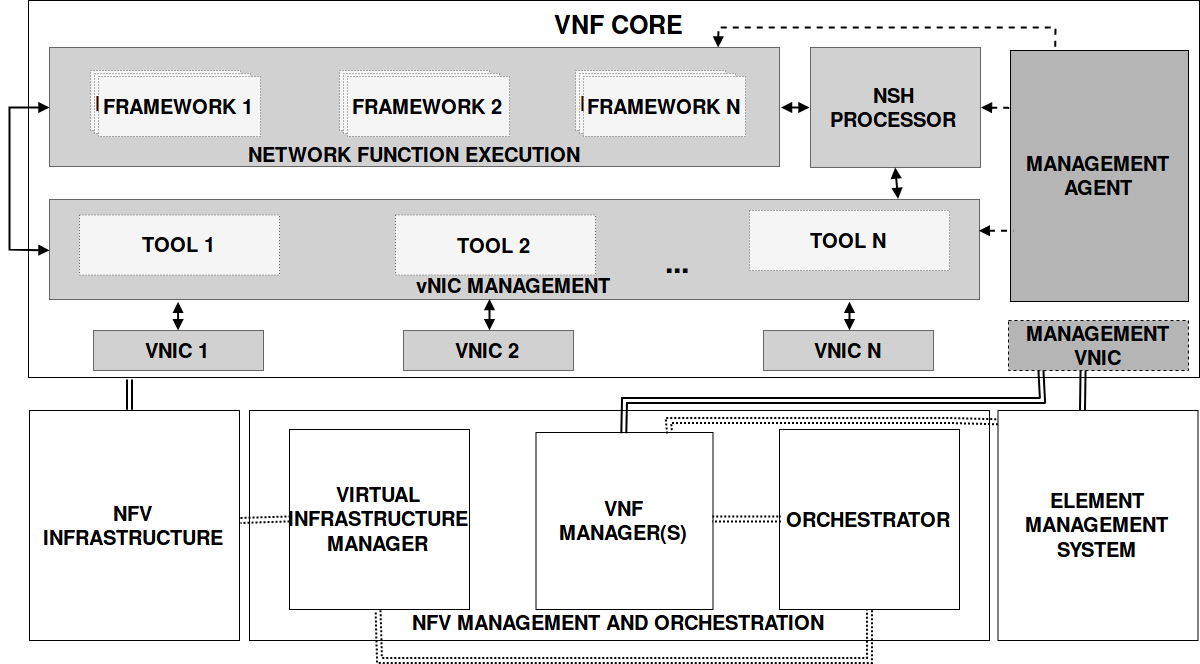
\includegraphics[width=\textwidth]{images/FullArchitecture_MOD.png}
    \caption{\label{vnfGeneric} VNF Platform Architecture}
\end{figure}

In this context, we propose a generic and flexible architecture for VNF platforms, (Figure~\ref{vnfGeneric}). The proposed platform consists of multiple modules, deployed on a host operating system (called here VNF Core): an module responsible for management access of Virtual Network Interfaces (vNIC), being the main point of input/output of packets from the architecture, a module consisting of a framework for development and execution of network functions, a management agent responsible for configuration of the host operating system and the other modules and, finally, a NSH Processor which provides an abstraction for the network functions regarding the existence of NSH packets.

% \blue{Packets I/O when executed by the native network stack in traditional operating systems, is not optimized to support the performance requirements of high-speed networks (\textit{e.g.}, 40GbE/100GbE). To tackle this problem, packet acceleration tools (\textit{e.g.}, Intel DPDK \cite{Intel-2014}, NetMap \cite{Rizzo-2012}) have been proposed and extensively evaluated. Once the network packets enter the VNF, they are forwarded internally through communication channels (\textit{e.g.}, using shared memory, pipes, sockets) to the NSH Processor if the VNF is in a service chain, otherwise being forwarded directly to the Network Functions.}

Network Service Header (NSH) is a new service plane protocol, specified by IETF, inserted onto packets/frames to provide service function paths \cite{Quinn-2018}. Despite its advantages, NSH is not always employed to steer traffic across multiple VNFs. In order to support the cases where NSH is employed or not, we introduced the NSH Processor, which is responsible for manipulating the NSH fields that may be modified when a packet is traversing a network path (\textit{i.e.,} the Service Index - SI; and Context Header - CH). The proposed NSHP also provides the following operations: NSH removal, NSH reinsertion, CH retrieval, and CH update.
% \blue{The IETF specified the Network Service Header (NSH) that is inserted in packets/frames to provide service function paths \cite{Quinn-2018}. However, despite its advantages, the use of NSH is optional to steer traffic across multiple VNFs. In order to support both cases, we define the NSH Processor, which acts on the specific NSH fields that may be modified when traversing a network path (\textit{i.e.,} the Service Index - SI; and Context Header - CH). NSHP provides the following operations: NSH removal, NSH reinsertion, CH retrieval, and CH update.}

Packets are then received by the development frameworks used to implement network functions. Basically, these frameworks include applications (\textit{e.g.}, Click Modular Router \cite{Kohler-2000} and Vector Packet Processing \cite{Cisco-2018}), programming languages (\textit{e.g.}, C, C++, Python), libraries (\textit{e.g.}, Scapy, libtins, libnet), or even single routines that support the construction and handling of network packets.

All the described modules are controlled by an management agent, which is responsible for monitoring and controling the execution of VNFs. Once a VNF is executing, the \textit{retrieve} operations can be used to gather information about the VNF instance (\textit{e.g.}, VNF ID, network interfaces), measuring performance indicators from the VNF Core (\textit{e.g.}, CPU, memory, and network usage), and providing information from the extended agents deployed in the VNF platform.

% upon receiving a configuration file, does the validation, extracts the relevant information for deploying the VNF, and

%The module is controlled by the Management Agent and is used to monitor/control each network function or component. It is supposed to be developed by the creator of the VNF/VNFC, as it acts on the individual management data of those implementations (\textit{e.g.}, number of discarded packets by a firewall). This module must provide at least one standard operation which we call ``list''. This operation is used by MA to discover all the management data that can be accessed by network operators.

%All the described modules are controlled by the MA, which upon receiving a VNFP (MA-MV interface), does the validation, extracts the relevant information for deploying the VNF, and configures the internal modules accordingly.


%For example, VNFP may contain information regarding the set of VNFCs that compose a VNF, which is essential for the Internal Router to forward the traffic to the proper components. The initial request for VNF deployment must also provide more specific information, such as the extended agents to be instantiated together with the network functions.

%The Management Agent is also responsible for extracting the implementation source code of the VNFCs from the VNFP, request the Packet Processing Subsystem to create the associated communication channels, and to start the execution of VNFCs (Figure \ref{vnfGeneric} MA-EA and PPSF-EA). Once this operation concludes, PPS returns a success/failure confirmation to the Management Agent (MA-PPS). In case of failures, rollback mechanisms may be employed to abort the instantiation process properly. When NSH is used, the Management Agent starts the NSH Processor (MA-NSHP). NSHP then creates a communication channel with the Packet Processing Subsystem (NSHP-PPS) to allow the network functions to access the NSH context header. VNICs are connected to the Virtual Network Subsystem (VNS-VNIC) based on the original request specified in the VNFP, processed by the MA (MA-VNS). The overall configuration of the VNF Platform is depicted in Figure \ref{FIG:CONF}.

%Finally, the Internal Router is initiated with two default communication channels: IR-VNS and IR-PPS. The former is used by the IR to retrieve network packets from the VNS, while the latter is used by VNFCs to access the packets to be processed. A third connection labeled IR-NSHP is used (i) to remove the NSH before any VNFC and (ii) to reinsert the NSH after the last VNFC of the path.

% \blue{The architecture described in this section defines modules responsible for the deployment of VNFs with SFC support\cite{Joel-2015}. We believe the architecture can provide a valuable reference for the design and development of VNF platforms, working as a guideline to integrate distinct modules in order to create complete solutions.}

\subsection{Prototype Development}\label{PROTO}

% Raniery (06/08): no geral a seção pode ser condensada em um texto mais limpo e direto. Por exemplo, a maior parte das explicações na segunda subseção já é mencionada antes. Na mesma linha, fiquei com a sensação de que alguns elements já são apresentados e discutidos na seção anterior. ACHO que toda a segunda subseção pode ser removida. Talvez algumas poucas partes possam migrar para outros lugares

%VINÍCIUS: Sim de fato, algumas coisas estão um pouco repetidas, porém aqui nos damos nomes aos bois, a idéia é justamente dizer, olha para tais e tais módulos, usamos tais e tais ténologias. Vou trabalhar com a idéia de não passar dados de relações e etc, mas de fato identificar detalhes de implementação.

% Raniery (06/08): Fiquei na dúvida se as informações estão consistentes ao longo da seção. Por exemplo fala sobre shared memory, L2 socket, L3 socket, system call.

%VINÍCIUS: Sim tudo é usado mesmo
%Shared Memory: comunicação entre os módulos internos a plataforma.
%L2 Socket: ferramenta de rede virtual para acessar as VNICs.
%L3 Scoket: Comunicação entre o PPS e os frameworks.
%System Call: Método de instanciação dos frameworks de processamento de pacotes

As a proof of concept of the proposed architecture presented in the previous section, we implemented a prototype that consists of a VNF platform that employs modern and well-accepted NFV enablers. In this context a NFV enabler is any technology used as a basis for the development of NFV ecosystems \cite{ETSI-2012}, such as hypervisors, packet acceleration frameworks, virtual routers, and operating systems.

\subsection{NFV enablers}

In our solution, we employ the following technologies:

% In this section we present a prototype based on the architecture previously defined in section \ref{ARCH}. The prototype was built on top of a Debian operating system (acting as VNF Core), while the internal modules were developed using modern NFV Enablers.
% In this section, a prototype based on the architecture previously defined in section \ref{ARCH} is presented. The prototype was built on top of a Debian operating system, with some components being specifically developed for the platform and others based on readily available frameworks. First, those frameworks (\textit{i.e.,} NFV Enablers), as well as the reasons of using they are briefly introduced. Then, the development process of the remaining components and how they interact with the enablers is presented. Finally, the interaction between those components inside the platform and with the NFV ecosystem is discussed.
% \subsection{NFV Enablers}
% An "NFV Enabler" is any technology that can be used as basis for the development of NFV ecosystems \cite{NFVPaper}, for example, hypervisors, packet acceleration frameworks, virtual routers, and operating systems. In the context of this paper, we have chosen the following technologies as basis for developed prototype, which aims to enable us in the analysis of the architectural design we presented previously. %, and analyze the NFV requirements and proposed modules of the   % For the platform development, some modules have functions that can be performed by already available frameworks, and due to the flexibility of the platform, they could be used to perform these functions, although this does not limits the usage of custom modules developed for the VNF.

\begin{itemize}
    \item \textbf{Click Modular Router} -- a well-known packet processing framework that provides an extensive list of network elements, native support for packet acceleration frameworks, and built-in control methods. The Click framework has been extensively investigated in academia and employed in several efforts to develop VNF platforms, such as ClickOS \cite{Martins-2014}, Click-on-OSv \cite{Marcuzzo-2018}, and the platform proposed by Bu \textit{et al.} \cite{Bu-2018}; % Click is used in our solution as the framework for packet processing (Python 3 is also supported), since its built-in elements enable the development of heterogeneous network functions and can be extended to support novel networking protocols.

      % \item \textbf{Click Modular Router}: the Click Modular Router is a well-known packet processing framework with an extensive list of network elements, native support for packet acceleration technologies, and built-in management methods. This framework was used in several efforts to develop VNF platforms, such as in \cite{clickos} and \cite{Bu-2018}. In the platform, it is used as the default packet processing framework, since its built-in elements make network function development easy for users (without having to implement the entire packet processing) and can also be extended to support new elements.

      \item \textbf{Intel Data Plane Development Kit (DPDK)} -- a packet acceleration framework that provides high throughput with reduced resource consumption (by using PCI passthrough and zero-copy) and supports multiple network interface cards (including paravirtualized ones, such as \texttt{virtio} and \texttt{netfront}); % DPDK was employed because it is one of the most widely accepted solutions today.

      % \item \textbf{Data Plane Development Kit}: the Intel Data Plane Development Kit (DPDK) is a packet acceleration framework, which is used as the default Virtual Network Subsystem, being capable of high performance with reduced resource usage, support for multiple different network interface cards (including paravirtualized ones such as virtio and netfront), as well as technologies such as polling, PCI passthrough and zero copy.

      \item \textbf{RESTful Web Services} -- an architectural style for the provisioning of Web Services (WSs) with simplified access to resources. RESTful web services are lighter than traditional SOAP-based WSs and are used here as the basis for the management agent to export performance statistics regarding the VNF platform, and to receive management requests from an external VNFM or EMS.

    % \item \textbf{RESTful Web Services}: an implementation of a REST Web Server is used for management and collection of statistics of the VNF platform. By using an Web API, the platform can be externally managed thorugh a dedicated management interface, detaching its management from the network where it is used to process packets.
\end{itemize}

Furthermore, we have chosen Debian as the operating system for the VNF Core. Although this operating system is not explicitly designed to support the NFV requirements (\textit{e.g.}, performance), this decision enabled us to focus on the development of the internal modules without concerns about software compatibility, thus enabling the analysis of the architecture from the functional point-of-view. However, the development of NFV platforms for production environments should benefit from more recent solutions such as  OSv, CoreOS, MiniOS, and Alpine.

% [ref1]: http://citeseerx.ist.psu.edu/viewdoc/download?doi=10.1.1.671.8671&rep=rep1&type=pdf

%\begin{figure*}[ht]
%\centering
%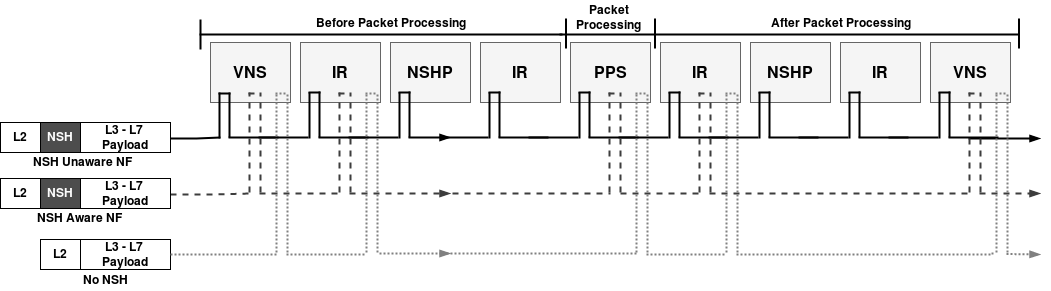
\includegraphics[width=.8\textwidth]{images/PlatformFlow.png}
%\caption{Prototype Platform Execution Scenarios}
%\label{FIG:PLATEXEC}
%\end{figure*}

\subsection{Platform Prototype}

% The platform was built on top of a minimal image of the operating system Debian 9. Packages were installed specifically to built an environment to provide the main functionalities of VNF systems introduced in the previous section. There are two main process in the platform: the data plane process and the management plane process. The VNFs platform architecture modules are implemented as sub-process, being the data plane process parent of the VNS, IR, NSHP, and PPS and the management plane process parent of the MA and EA.

For handling the vNICs, we initially chose DPDK. However, the platform also supports L2 Sockets to provide increased flexibility. These two options are available and can be selected according to the specific needs of the operator\footnote{The polling method of DPDK is inefficient regarding to CPU resources, while L2 Sockets are not able to achieve high throughput.}. Although we have employed these two solutions, other solutions (\textit{e.g.}, PF\_RING, and netmap) could be used without significant implementation efforts.

% The Virtual Network Subsystem is provided by two tools: the DPDK and L2 sockets. These tools are used to receive network packets from the virtualized interfaces and forward them to the internal router. Although only the DPDK and L2 sockets were made available in the platform, any framework compatible with Linux and with paravirtualized network drivers, such as netmap and PF\_RING, could be inserted in the platform and provided for the VNFs developers with minimum programming efforts.
%VINICIUS: fiz alterações aqui, o Internal Router não tem duas opções de comunicação, mas sim, um tipo para módulos internos e outro para os módulos externos, aqui a escrita passou a ideia errada do que realmente acontece na implementação.

%The Internal Router communicates with other internal modules of the architecture (\textit{i.e.}, Virtual Network Subsystem and NSH Processor) on shared-memory to guarantee high performance. For the communication with PPS (\textit{i.e.} NFs or VNFCs), L3 Sockets are employed, which may affect the latency and throughput when compared to shared memory. However, L3 Sockets provide greater flexibility in the development of NFs and VNFCs.

%platform independence during the NF (or VNFCs) development and a higher compatibility with current NFs implementations.}

%The Internal Router can communicate with other internal modules of the architecture (e.g., NSHP and MA) by using shared memory or conventional L3 Sockets. The prior provides greater performance, however doesn't allow the internal modules to be decoupled from the VNF platform (i.e., be executed outside the user space), while the later may affect latency. Shared memory is also used for communication between multiple VNFCs, while sockets are used by the NFs to receive/send network packets from/to the IR.

% forward packets to the individual VNFCs by using shared memory or conventional L3 Sockets. The prior provides greater performance, however doesn't allow the internal modules to be decoupled from the VNF platform (i.e., be executed outside the user space), while the later may affect latency. Shared memory is also used for  inter-related process communication between the IR and the Management Agent.
% The Internal Router is responsible for forwarding packets to the other VNF platform modules, ensuring they arrive at the correct destination. As such, it can forward packets by using shared memory areas (preferred due to its performance, however requires modifications on external modules) or by using sockets, achieving greater compatibility but typically with an extra delay. The prototype internal data plane modules are implemented supporting inter-process memory sharing which is used to perform the communication. In the other hand, the NFs deployed in the platform communicates the Internal Router through generic L3 sockets, being platform agnostic (\textit{i.e.}, the functions can be used in other platforms without any modification).

The NSH Processor operates as a proxy during the platform execution and can be enabled by the network operator. When enabled, packets first pass through the NSHP in order to remove NSH before steering the packets to the network function (\textit{i.e.}, CMR or Python-based NFs/VNFCs), and for NSH reinsertion before forwarding processed packets back to the vNIC (\textit{i.e.}, DPDK or L2 Sockets). The NFs, when necessary, can access the NSH Context Header to retrieve or replace content using specific libraries we developed (both in Python and CMR)\footnote{By the time of writing, we opted to support only Context Headers of fixed-length \cite{Quinn-2018}.}. Notice that, during the NSHP reinsertion operation, the Service Index field is updated.

%the NSHP removes the NSH specific header from each network packet prior delivering them to Packet Processing Subsystem (i.e., the NFs), and reinserts it before sending to the Virtual Network Subsystem (i.e., DPDK or L2 Socket). The NFs, when necessary, can access the NSH's Context Header to retrieve or replace its content by using specific functions (both in Python and CMR) we developed to enable these operations. \footnote{By the time of this work, we opted to support only Context Headers of fixed-lenght \cite{rfc8300}}. It's important to notice that, prior reinserting the NSH, the Service Index field is updated by the NSHP.

% Finally, after the packets are processed by the PPS, the Service Index field is updated and the data is encapsulated back to the NSH.

%As for the NSH Processor, it was developed as an optional activation element in the platform prototype. The NSH Processor acts like a proxy during the platform execution. When this module is active, before the packets be steered for the Packet Processing Subsystem, they are processed in order to remove and keep the NSH. Every processed packet is marked in order to identify it during the NSH reinsertion process. The NFs, when necessary, can request the NSH's Context Header retrieving or replacement through an standard REST interface provided by the NSHP. The prototype NSH Processor module works with fixed-length Context Headers \cite{rfc8300}. Finally, after the packets processing by the PPS, the IR forwards them for the NSHP in order to update the Service Index and reinsert the header.

% The Packet Processing Subsystem, in the platform, supports network functions implemented both in Click Modular Router (CMR) and Python 3. It hosts a single NF, but it can be instantiated as a set of components. These components can be independent from each other once all the traffic steering between them are made by the Internal Router. Due this independence, components implemented using different frameworks can natively cooperate to provide an entire network function.

% Raniery (06/09): senti falta de uma figura nesta seção para explicar melhor o conceito de NSH. Pensei algo semelhante a estas:
% - http://meetings.ripe.net/ripe-42/presentations/ripe42-eof-pseudowires2/sld011.html
% - https://blogs.cisco.com/sp/making-software-defined-networks-work-for-the-service-providers-success
% - https://www.slideshare.net/OPNFV/opnfv-service-function-chaining (slides 6 e 7)
% Estilo de imagem: https://docs.opnfv.org/en/stable-fraser/submodules/sfc/docs/development/design/architecture.html

The Management Agent was developed as a RESTful WS and is able to control (through system calls and CMR's control socket) all the internal components of the platform. For monitoring, Glances\footnote{https://nicolargo.github.io/glances/} was used to recover system-wide statistics, while a custom REST API was developed to meet the management requirements as specified in \cite{Bondan-2014}, such as providing information regarding the VNF (\textit{e.g.}, function description, system state, logs) and supporting the reconfiguration of running functions. These operations can be accessed either directly by network operators (through the integrated EMS) or by external EMS and VNF Managers (by using REST calls to the management interface).

To initiate the platform, the network operator must first provide (through the Management Agent) a VNF Package that contains the network function implementation, its descriptor, and settings to initialize the internal modules properly. These settings are used, for example, to configure the Internal Router with the VNFC chaining order and to enable/disable the NSH Processor. After the initial platform configuration, the NF lifecycle operations (\textit{e.g.}, start, stop, status, and monitoring) become available to the network operator. The platform prototype supports three execution scenarios: NSH packets with NSH unaware NF, NSH packets with NSH aware NF, and packets without NSH.

% Finally, the management agent was developed as a RESTful WS, able to both control (through system calls and CMR's control socket) all the internal components of the platform. For monitoring, Glances was used to recover system-wide statistics, while a custom REST API was developed in order to meet the management requirements detailed in \cite{manRequirements}, such as providing information regarding the VNFs (textit{e.g.}, function description, system state, logs) and supporting the reconfiguration of running functions. These operations can be accessed either directly by the network operators (through the integrated EMS) or by external EMS and VNF Managers (by using REST calls to the management interface).

%\subsection{Interconnection between modules}

% Before the platform can start operation, the NFV Orchestrator or a user must provide a configuration file containing the network function and the modules initialization routines. The platform receives this descriptor and configure its internal connections in order to allow the execution of the function.

% The (VNS-VNIC) connections can be set up by a L2 socket or by the DPDK packet acceleration tool. The (IR-VNS), (IR-NSHP), and (IR-PPS) connections are implemented using inter-process shared memory. The race conditions related to the shared memory writing is treated by using mutexes. The (NSHO-PPS) consists of a REST interface to request NSH Context Header operations. Every connection related to the management plane (\textit{i.e.}, (MA-PPS), (MA-EA), (PPSF-EA), (MA-NSHP), (MA-IR), (MA-VNS), and (MA-MV)) are also created using REST interfaces.

%Except for inter-VNFC communication, all the network packets arriving the NIC are directly captured by the Virtual Network Subsystem, which forwards those packets to the Internal Router through an internal socket. If NSH processing is opted by the network operator, the packets are first delivered to the NSH Processor before being processed by the Packet Processing Subsystem. In the other case, the NSHP is bypassed and packets are directly delivered to the proper NF/VNFC.

% Except in functions where traffic is generated from inside the VNF, packets always enter through a NIC going to the Virtual Network Subsystem, which then forwards those packets to the internal router through a internal socket. On the internal router, if NSH processing is required by the function, it forwards traffic to the NSH processor, which perform its required operations before forwarding traffic to the Packet Processing Subsystem. This step is bypassed if the function do not requires NSH processing. Inside the Packet Processing Subsystem, the packet is then processed and sent to another framework for post-processing, or back to the internal router, if it is a outgoing packet. Once the router receives this packet, it forwards it to the Virtual Network Subsystem which sends the processed packet to the network.
